\chapter{无穷积分}

\begin{theorem}{比较判别法}
	$\forall x\in [a,+\infty)$,有$|f(x)|\le c\varphi (x)$(c是正常数).
	\begin{enumerate}
		\item 若无穷积分$
			      \int_a^{+\infty}{\varphi \left( x \right) \text{d}x}
		      $收敛,则无穷积分$
			      \int_a^{+\infty}{f \left( x \right) \text{d}x}
		      $也收敛;
		\item 若无穷积分$
			      \int_a^{+\infty}{|f \left( x \right)| \text{d}x}
		      $发散,则无穷积分$
			      \int_a^{+\infty}{\varphi \left( x \right) \text{d}x}
		      $也发散;
	\end{enumerate}
\end{theorem}

\begin{theorem}{Cauchy判别法}
	$\forall x\in [a,+\infty),f(x)>0$,且$
		\lim\limits_{x\rightarrow +\infty}x^pf\left( x \right) =d
	$,$d \in [0,+\infty)$.
	\begin{enumerate}
		\item 若$p>1,0\le d<+\infty$,则无穷积分$
			      \int_a^{+\infty}{f \left( x \right) \text{d}x}
		      $收敛;
		\item 若$p\le 1,0< d\le+\infty$,则无穷积分$
			      \int_a^{+\infty}{f \left( x \right) \text{d}x}
		      $发散;
	\end{enumerate}
\end{theorem}

\begin{theorem}{Abel判别法}
	设函数$f(x)$在$[a,+\infty)$上单调有界,$
		\int_a^{+\infty}{g \left( x \right) \text{d}x}
	$收敛,则无穷积分$
		\int_a^{+\infty}{f(x)g \left( x \right) \text{d}x}
	$收敛
\end{theorem}

\begin{theorem}{Dirichlet判别法}
	设函数$f(x)$在$[a,+\infty)$上单调且$
		\lim\limits_{x\rightarrow +\infty}f\left( x \right) =0
	$,积分$
		\int_a^{A}{g \left( x \right) \text{d}x}
	$($A>a$)有界则无穷积分$
		\int_a^{+\infty}{f(x)g \left( x \right) \text{d}x}
	$收敛
\end{theorem}

\begin{example}
	(Froullani积分) 设函数$f(x)$在$[0,+\infty)$上连续,$f(+\infty)$存在且有限,实数$a$,$b>0$,计算积分
	$$
		J=\int_0^{+\infty}{\frac{f\left( ax \right) -f\left( bx \right)}{x}dx}
	$$
\end{example}

\begin{proof}
	(收敛性的证明包含在下面的计算过程中)对任意的$0<r<R<+\infty$,由定积分的换元公式,有
	$$
		\int_r^R{\frac{f\left( ax \right) -f\left( bx \right)}{x}dx}=\int_r^R{\frac{f\left( ax \right)}{x}\text{d}x}-\int_r^R{\frac{f\left( bx \right)}{x}\text{d}x}
	$$
	$$
		=\int_{ar}^{aR}{\frac{f\left( x \right)}{x}\text{d}x}-\int_{br}^{bR}{\frac{f\left( x \right)}{x}\text{d}x}
	$$
	由积分中值定理,存在$\xi \in (ar,br),\eta \in (aR,bR)$,使得
	$$
		\int_r^R{\frac{f\left( ax \right) -f\left( bx \right)}{x}dx}=f\left( \xi \right) \int_{ar}^{br}{ \frac{\text{d}x}{x}-f\left( \eta \right)}\int_{aR}^{bR}{\frac{\text{d}x}{x}}=\left[ f\left( \xi \right) -f\left( \eta \right) \right] \ln \frac{b}{a}
	$$
	令$r \rightarrow 0^+,R \rightarrow +\infty$,得
	$$
		J=\left[ f\left( 0 \right) -f\left( +\infty \right) \right] \ln \frac{b}{a}
	$$
\end{proof}

\begin{example}
	(Dirichlet积分) 证明:$
		\int_0^{+\infty}{\frac{\sin x}{x}\text{d}x}=\frac{\pi}{2}
	$
\end{example}

\begin{proof}
	\begin{enumerate}
		\item 收敛性的证明.由于$
			      \lim\limits_{x\rightarrow 0^+}\frac{\sin x}{x}=1
		      $,故$x=0$不是被积函数的瑕点.一下只需要证明$\int_1^{+\infty}{\frac{\sin x}{x}\text{d}x}$收敛.因$
			      \left| \int_1^A{\sin x\text{d}x} \right|\le 2
		      $,$
			      \frac{1}{x}
		      $在$[1,+\infty)$上严格减少且$\lim\limits_{x\rightarrow +\infty}\frac{1}{x}=0$,由Dirichlet判别法知,$\int_1^{+\infty}{\frac{\sin x}{x}\text{d}x}$收敛,从而$\int_0^{+\infty}{\frac{\sin x}{x}\text{d}x}$也收敛(实际上$\int_0^{+\infty}{\frac{\sin x}{x}\text{d}x}$条件收敛).
		\item 等式的证明.我们知道,
		      $$
			      \int_0^{\pi}{\frac{\sin \left( n+\frac{1}{2} \right)x}{2\sin \frac{x}{2}}\text{d}x}=\int_0^{\pi}{\left( \frac{1}{2}+\sum_{k=1}^n{\cos kx} \right) \text{d}x=\frac{\pi}{2}}
		      $$
		      利用含参量积分的性质,有
		      $$
			      \lim_{n\rightarrow \infty}\int_0^{\pi}{\frac{\sin \left( n+\frac{1}{2} \right) x}{x}\text{d}x}=\lim_{n\rightarrow \infty}\int_0^{\pi}{\left[ \frac{\sin \left( n+\frac{1}{2} \right) x}{2\sin \frac{x}{2}}\cdot \frac{2\sin \frac{x}{2}}{x} \right] \text{d}x}
		      $$
		      $$
			      =\int_0^{\pi}{\lim_{n\rightarrow \infty}\frac{\sin \left( n+\frac{1}{2} \right) x}{2\sin \frac{x}{2}}\text{d}x}=\lim_{n\rightarrow \infty}\int_0^{\pi}{\frac{\sin \left( n+\frac{1}{2} \right) x}{2 \sin \frac{x}{2}}\text{d}x}
		      $$
		      $$
			      =\lim_{n\rightarrow \infty}\frac{\pi}{2}=\frac{\pi}{2}
		      $$
		      再由换元积分法,得
		      $$
			      \frac{\pi}{2}=\lim_{n\rightarrow \infty}\int_0^{\pi}{\frac{\sin \left( n+\frac{1}{2} \right) x}{x}\text{d}x}=\lim_{n\rightarrow \infty}\int_0^{\left( n+\frac{1}{2} \right) \pi}{\frac{\sin x}{x}\text{d}x}=\int_0^{+\infty}{\frac{\sin x}{x}\text{d}x}
		      $$
	\end{enumerate}
\end{proof}

\begin{note}
	对收敛的广义积分(包括无穷积分与瑕积分),可以使用Newton-Leibniz公式.当然在将积分上下限代入所得的"部分原函数"时,需用对应的极限代替函数值.例如
	$$
		\frac{1-\cos x}{2x}\mid_{0}^{+\infty}=\lim_{x\rightarrow \infty}\frac{1-\cos x}{2x}-\lim_{x\rightarrow 0^+}\frac{1-\cos x}{2x}=0
	$$
\end{note}

下面是无穷积分在无穷远的性质.

\begin{example}
	设$f(x)$在$[a,+\infty)$上一致连续,且$
		\int_0^{+\infty}{f\left( x \right) dx}
	$收敛,则$
		\lim\limits_{x\rightarrow +\infty}f\left( x \right) =0
	$.
\end{example}

\begin{proof}
	因为$f(x)$在$[a,+\infty)$上一致连续,对任意$\varepsilon >0$,存在$\delta >0$(不妨设$\delta < \varepsilon$),使得对任何$x_1,x_2 \in [a,+\infty)$,只要$|x_1-x_2|<\delta$,就有
	$$
		\left| f\left( x_1 \right) -f\left( x_2 \right) \right|<\frac{\varepsilon}{2}
	$$
	又由$
		\int_0^{+\infty}{f\left( x \right) dx}
	$收敛,所以存在$T>a$,使得任意$x_1,x_2>T$,有$$
		\left| \int_{x_1}^{x_2}{f\left( x \right) \text{d}x} \right|<\frac{\delta ^2}{2}
	$$
	于是对任意$x>T+\frac{\delta}{2}$,取$x_1=x-\frac{\delta}{2},x_2=x+\frac{\delta}{2}$,则
	$$
		\left| f\left( x \right) \right|\delta =\left| \int_{x_1}^{x_2}{f\left( x \right) \text{d}t}-\int_{x_1}^{x_2}{f\left( t \right) \text{d}t}+\int_{x_1}^{x_2}{f\left( t \right) \text{d}t} \right|\le
	$$
	$$
		\int_{x_1}^{x_2}{\left| f\left( x \right) -f\left( t \right) \right|\text{d}t+\left| \int_{x_1}^{x_2}{f\left( t \right) \text{d}t} \right|}<\frac{\varepsilon \delta}{2}+\frac{\delta ^2}{2}
	$$
	从而$
		\left| f\left( x \right) \right|<\frac{\varepsilon}{2}+\frac{\delta}{2}<\varepsilon
	$,故$
		\lim\limits_{x\rightarrow +\infty}f\left( x \right) =0
	$.
\end{proof}

\begin{example}
	证明:若$f(x)$连续可微,积分$
		\int_a^{+\infty}{f\left( x \right) dx}
	$和$
		\int_a^{+\infty}{f'\left( x \right) dx}
	$都收敛,则$x \rightarrow +\infty$时,有$f(x) \rightarrow 0$.
\end{example}

\begin{proof}
	要证明当$x \rightarrow +\infty$时,有$f(x)$有极限,只要证明$
		\forall \left\{ x_n \right\} \rightarrow +\infty
	$恒有$\left\{f(x_n)\right\}$收敛.事实上,因为$
		\int_a^{+\infty}{f'\left( x \right) dx}
	$收敛,据Cauchy收敛准则,对任意$
		\forall \varepsilon >0
	$,存在$A>a$,当$x_1,x_2>a$时,恒有$
		\left| \int_{x_1}^{x_2}{f'\left( x \right) \text{d}x} \right|<\varepsilon
	$.那么$
		\forall \left\{ x_n \right\} \rightarrow +\infty
	$,存在$N>0$,当$n,m>N$,有$x_n,x_m>A$,从而$$
		\left| \int_{x_n}^{x_m}{f'\left( x \right) \text{d}x} \right|=\left| f\left( x_n \right) -f\left( x_m \right) \right|<\varepsilon
	$$因此恒有$\left\{f(x_n)\right\}$收敛,从而极限$
		\lim\limits_{x\rightarrow +\infty}f\left( x \right) =a
	$存在.

	下面证明$a=0$.若$a>0$,则由保号性,存在$M>0$,当$x>M$时,有$f(x)>\frac{a}{2}>0$,从而$A>M$时$
		\left| \int_A^{2A}{f\left( x \right) \text{d}x} \right|\ge \frac{a}{2}A\rightarrow +\infty
	$(当$A\rightarrow +\infty$时).这与$
		\int_a^{+\infty}{f\left( x \right) dx}
	$收敛矛盾.同理可证$a<0$也不可能,故$
		\lim\limits_{x\rightarrow +\infty}f\left( x \right) =a=0
	$
\end{proof}

\begin{example}
	(第十五届全国大学生数学竞赛数学B类)设非负函数$f$在$[0,+\infty)$上连续可微,无穷积分有$
		\int_{0}^{+\infty}{f\left( x \right) \text{d}x}
	$收敛,且存在$[0,+\infty)$上的非负函数$g$,使得
	$$f'(x) \le g(x),x\ge 0$$
	分别就下列三种情形,证明$
		\lim\limits_{x\rightarrow +\infty}f\left( x \right) =0
	$.
	\begin{enumerate}
		\item $
			      \int_{0}^{+\infty}{g\left( x \right) \text{d}x}
		      $收敛.
		\item $g(x)=C>0$,其中C为常数.
		\item $g(x)=Cf^p (x)$,其中$C>0,p>0$为常数.
	\end{enumerate}
\end{example}

\vspace*{7cm}

\begin{example}
	证明:$I=\int_0^{+\infty}{e^{-x^2}\text{d}x}=\frac{\sqrt{\pi}}{2}$.
\end{example}

\begin{note}
	对于本题直接去算是算不出来的,所以需要利用二重积分构造圆环使用面积关系去逼近,具体面积关系如下图所示\\
	\begin{center}
		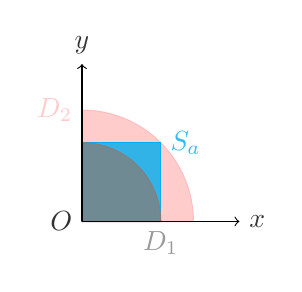
\begin{tikzpicture}[fill opacity=0.8]
			\filldraw[pink] (1.414,0) arc (0:90:1.414) --(0,0) --(1.414,0) arc (0:90:1.414) node[left] {$D_2$};
			\filldraw[cyan][-] (1,0) --(1,1) --(0,1) --(0,0);
			\draw[cyan] (0,0) --(0,1) --(1,1) --(1,0) --(0,0) --(0,1) --(1,1) node[right] {$S_a$};
			\filldraw[gray] (1,0) arc (0:90:1) --(0,0) --(1,0) node[below] {$D_1$};
			\draw[->] (0,0) --(2,0) node[right] {$x$};
			\draw[->] (0,0) --(0,2) node[above] {$y$};
			\draw (0,0) node[left] {$O$};
		\end{tikzpicture}
	\end{center}
\end{note}

\begin{proof}
	设$$S_a=[0,a]\times[0,a]$$显然$f(x,y)=e^{-(x^2+y^2)}$在$S_a$上可积,且
	$$
		F\left( a \right) =\iint_{S_a}{e^{-\left( x^2+y^2 \right)}dxdy}=\int_0^a{e^{-x^2}dx}\int_0^a{e^{-y^2}dy}=\left( \int_0^a{e^{-x^2}dx} \right) ^2
	$$
	作半径为$a$和$\sqrt{2}a$的$\frac{1}{4}$的圆$D_1$和$D_2$,使得$$D_1\subset S_a\subset D_2$$由$e^{-\left( x^2+y^2 \right)}>0$有
	$$
		H\left( a \right) =\iint_{D_1}{e^{-\left( x^2+y^2 \right)}dxdy}\le F\left( a \right) \le \iint_{D_2}{e^{-\left( x^2+y^2 \right)}dxdy}=G\left( a \right)
	$$
	而
	$$
		H\left( a \right) =\iint_{D_1}{e^{-\left( x^2+y^2 \right)}dxdy}=\int_0^{\frac{\pi}{2}}{\int_0^a{e^{-r^2}rdrd\theta}}=\frac{\pi}{4}\left( 1-e^{-a^2} \right)
	$$
	类似有$
		G\left( a \right) =\frac{\pi}{4}\left( 1-e^{-a^2} \right)
	$,且有
	$$
		\lim_{a\rightarrow +\infty}H\left( a \right) =\lim_{a\rightarrow +\infty}G\left( a \right) =\frac{\pi}{4}
	$$
	由夹逼原则可得
	$$
		\lim_{a\rightarrow +\infty}F\left( a \right) =\lim_{a\rightarrow +\infty}\left( \int_0^a{e^{-x^2}dx} \right) ^2=\frac{\pi}{4}
	$$
	所以
	$$
		I=\int_0^{+\infty}{e^{-x^2}dx}=\frac{\sqrt{\pi}}{2}
	$$
\end{proof}
